\documentclass{book}
\usepackage{graphicx} % Required for inserting images

\usepackage[utf8]{inputenc}
\usepackage[T1]{fontenc}
\usepackage{listings}
\usepackage{appendix}
\usepackage{siunitx}
\usepackage{multirow}
\usepackage{mhchem}
\usepackage{natbib}
\usepackage{booktabs}
\DeclareSIUnit\msun{\text{M\ensuremath{_\odot}}}
\usepackage{astrojournals}
\bibliographystyle{aasjournal}
\renewcommand{\lstlistingname}{Algoritmus}

\title{Avances de tesis}
\author{r.reyes }
\date{December 2023}

\begin{document}

\maketitle

\tableofcontents

\newpage

\chapter{Introducción}

Los \text{glóbulos} son grandes concentraciones de gas y polvo en el medio interestelar que se cree que se forman por inestabilidades térmicas, colapso gravitacional o turbulencia. Estos glóbulos se pueden formar en regiones de formación estelar masiva o en nebulosas alrededor de estrellas evolucionadas y en realidad tienen muchos tamaños.

Cuando nos referimos a los glóbulos en regiones de formación estelar masiva, estos tienden a ser de un gran tamaño comúnmente, $\sim$\SI{0.1}{pc}, e interactúan con la radicación UV (ultravioleta) de las estrellas jóvenes masivas como estrellas tipo O, mientras que en nebulosas alrededor de estrellas evolucionadas son de un tamaño más pequeño, $\sim$\SI{e-2}{pc}. En algunos casos dependiendo que tan intensa es la radiación incidente por parte de la o las estrellas, podemos ver un \textit{flujo fotoevaporativo} por parte del glóbulo, el cual es causado por la radiación incidente.

Los primeros glóbulos fueron observados por Bart Bok en 1940, estos glóbulos son nubes oscuras, relativamente pequeños comparados con otras regiones de formación estelar, que tienen gran cantidad de gas y polvo. Estos glóbulos contienen principalmente hidrógeno molecular en su interior, así como también pueden tener otras moléculas, metales e incluso algunos silicatos. Si bien puede tener formación estelar en su interior no podemos ver la radiación de las estrellas ya que es absorbida por el hidrógeno atómico y el polvo, es por eso que se ven oscuras. Sin embargo, estos pueden ser radiados externamente, en regiones de formación estelar, por estrellas jóvenes masivas que se están formando cerca, y en algunos casos podemos ver el frente de ionización.

\begin{figure}[h!]
    \centering
    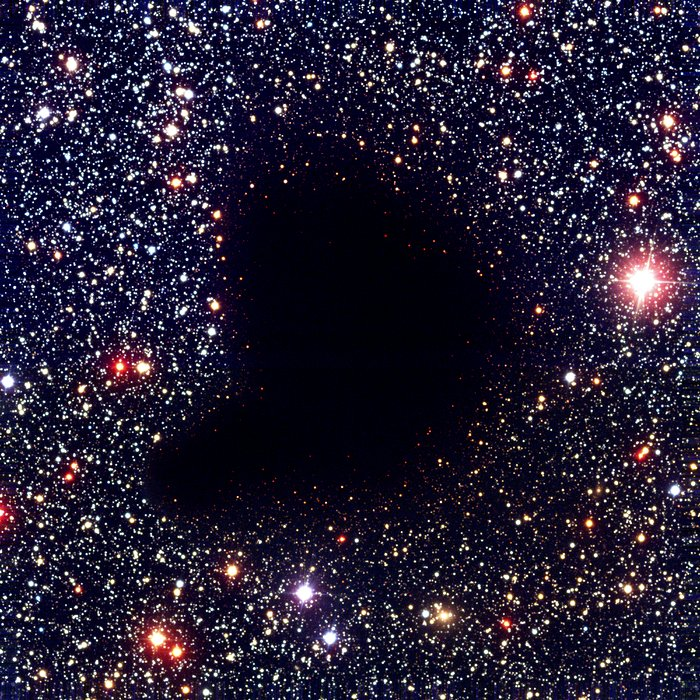
\includegraphics[width=0.75\textwidth]{images Chapter 1/C1_Bok_globule.jpg}
    \caption{Imagen de Banard 68, un ejemplo de un glóbulo de Bok, visto con Very Large Telescope FORS1 en 440 nm, 557 nm y 768 nm. Se puede apreciar una zona oscura y lo que pareciera ser enrojecimiento de las estrellas por polvo en la superficie del glóbulo. En esta imagen podemos ver que no hay evidencia de alguna fotoevaporación externa por parte de estrellas. \citep{Alves:2001}.}
    \label{fig:Banard}
\end{figure}

Esta interacción entre estrellas y glóbulos se puede dar a diferentes escalas, lo que nos da una gran variedad de estructuras. Entre las de mayor tamaño se encuentran lo que parecen ser columnas, pilares o trompas de elefantes, como se les conoce en la literatura, que llegan a tener un tamaño de $\sim$\SI{1}{pc} y una densidad del orden de \SI{e3}{cm^{-3}}. En algunas ocasiones tienden a llamar glóbulo en la literatura a los que, al igual que lo anterior a mencionado, tienen una gran estructura también pero son más densos, $\sim$ \SI{e4}{cm^{-3}}. Esta interacciones también se puede dar dentro de regiones HII, como vemos en la figura \ref{fig:Pillars}.

\begin{figure}[h]
    \centering
    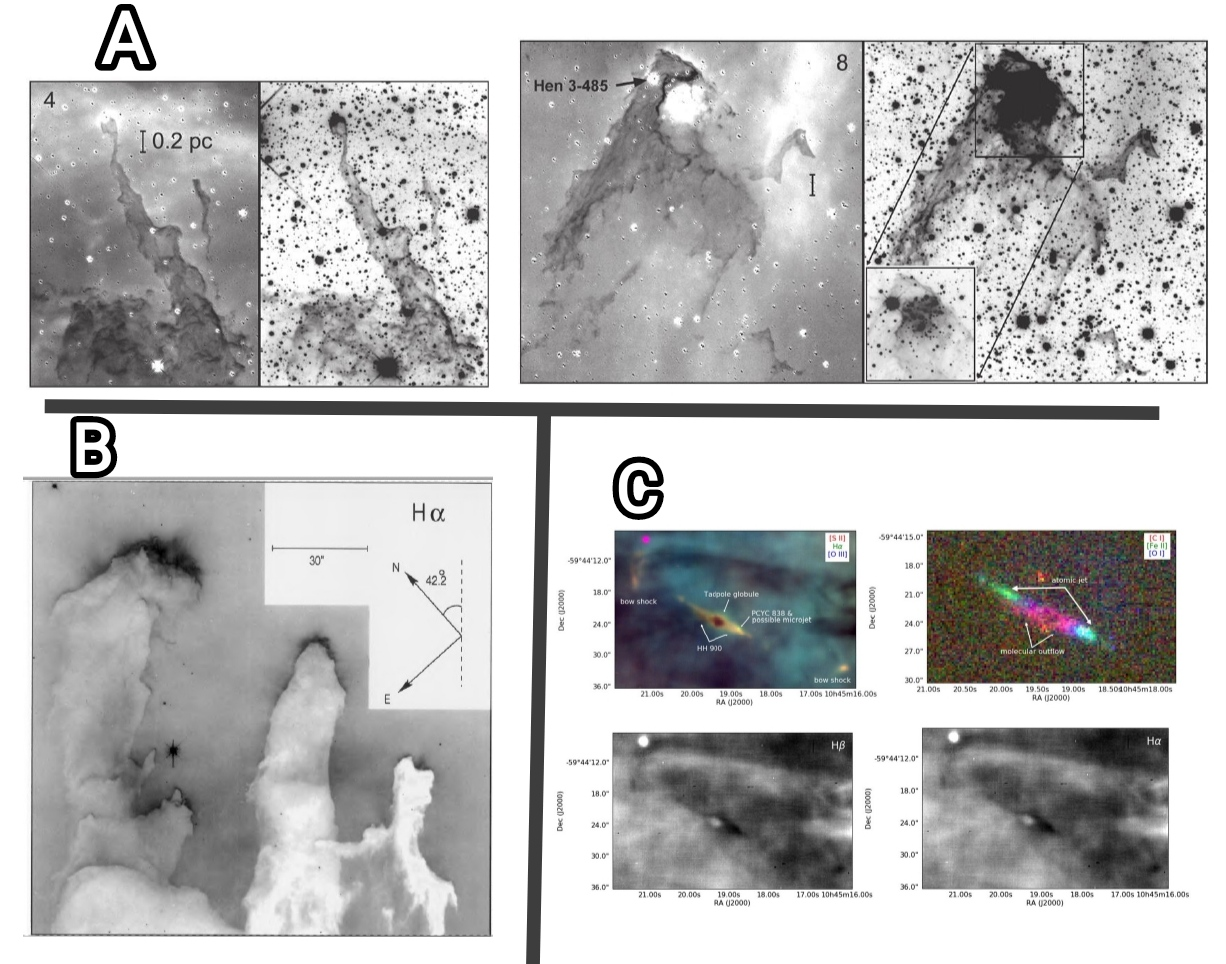
\includegraphics[width=1 \textwidth]{images Chapter 1/C1_Pillars.jpg}
    \caption{En \textbf{A} vemos dos ejemplos de pilares, donde la imagen derecha de cada ejemplo es vista a 2.12$\mu$m (\SI{}{H_2}), y la imagen izquierda es \SI{}{H_2-Br_{\gamma}} \citep{Hartigan:2015}. \textbf{B}, ejemplo de una trompa de elefante, es una imagen de M16 tomada con WFPC2 con e filtro F656N, los \SI{30}{\arcsecond} corresponden \SI{9e17}{cm} (\SI{0.29}{pc}) \citep{JJHester:1996}. \textbf{C} es el outflow de Tadpole globule, el cual consta del sistema HH900 jet+outflow, la imagen de abajo es vista en \SI{}{H_\alpha} con el continuo 
    \citep{MeganReiter:2019}. }
    \label{fig:Pillars}
\end{figure}

En escalas más pequeñas están lo que se conoce como EGGs (Evaporating Gaseous Globule), en escalas de $\sim$\SI{0.1}{pc}, y los proplyds, en escalas de $\le\SI{e-2}{pc}$. 

No solo se da en regiones de formación estelar, como ya hemos dicho, también hay dentro de nebulosas alrededor de estrellas evolucionadas donde se les conoce más comúnmente como \textit{nudos}, un ejemplo de esto es la imagen \textbf{D} de la figura \ref{fig:nudos}. Estos nudos son los que estudiaremos más fondo en este trabajo.

\begin{figure}[h]
    \centering
    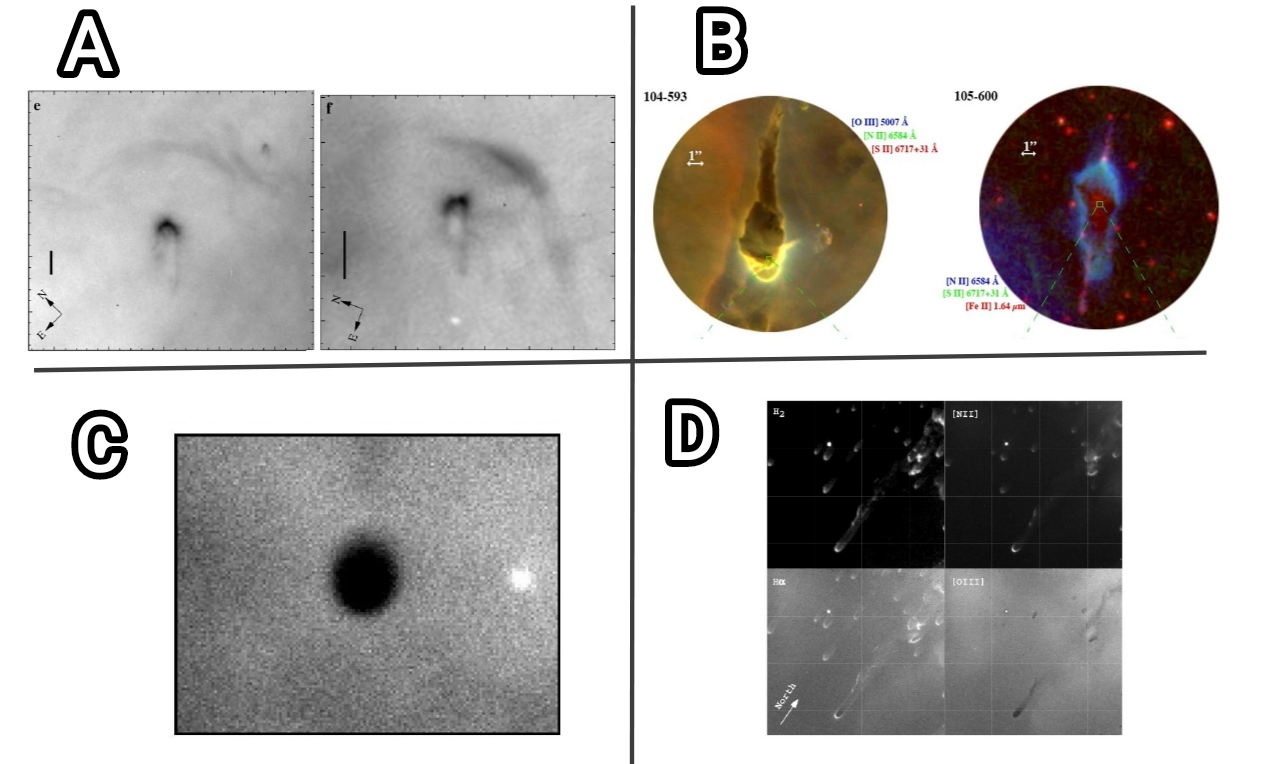
\includegraphics[width=1 \textwidth]{images Chapter 1/C1_Globulettes.jpg}
    \caption{En \textbf{A} vemos proplyds con su bowshock en Orion tomado con HST planetary camera, la barra negra indica una medida de \SI{1}{\arcsecond} que corresponde a 430 AU (\SI{2e-3}{pc}) \citep{Garcia-Arredondo:2001}. \textbf{B} son ejemplos de EGGs en Carina, tomado con WFC3, ACS, WFPC2 \citep{Mesa-Delgado:2016}. \textbf{C} es el globulette denso RN88 visto en \SI{}{H_\alpha} con un diámetro de \SI{6}{\arcsecond} (\SI{4e-2}{pc}) en la nebulosa de Rosette \citep{GFGahm:2013}. \textbf{D} son ejemplos de nudos en la nebulosa de la Hélice, los mosaicos tienen una medida de \SI{47.5}{\arcsecond}$\times$\SI{44.8}{\arcsecond} (\SI{4.76e-2}{pc}$\times$\SI{4.49e-2}{pc}) \citep{O'Dell:2007}. }
    \label{fig:nudos}
\end{figure}



\section{Flujos de foto evaporación ionizada} \label{Sec:fluijos fotoevaporativos}

Todos los ejemplos de las figuras \ref{fig:Banard}, \ref{fig:Pillars} y \ref{fig:nudos} se encuentran ya sea en regiones de formación estelar o en nebulosas alrededor de estrellas evolucionadas. 

Lo interesante en todos estos ejemplos es la forma que toman al interaccionar con las estrellas más masivas que se encuentran cerca, esto para los glóbulos que se encuentran en regiones de formación estelar.  Mientras que los que se encuentran en nebulosas planetarias, interactúan con la estrella evolucionada. Durante estas interacciones en algunos casos podemos ver lo que se conoce como flujos fotoevaporativos, los cuales explicaremos mejor a continuación.

Para que se pueda dar esta interacción y crear un flujo fotoevaporativo por parte de la nube es necesario que la estrella ionizante sea masiva o tenga un gran flujo ionizante como para poder ionizar el gas neutro. \cite{OortySpitzer_1955} explican a manera detallada como es la interacción entre una estrella tipo O y una nube interestelar de gas neutro. Con esto podemos explicar de una mejor manera como es la interacción en regiones de formación estelar masiva. Recordemos que en las regiones de formación estelar hay michas estrellas nuevas que emiten principalmente en radio o infrarrojo, por lo que no todas las estrellas nuevas pueden ionizar el gas neutro.

\cite{OortySpitzer_1955} consideran tres partes importantes para esto, la estrella ionizante, la nube interestelar de gas neutro y la región que hay entre la estrella y la nube interestelar. La nube interestelar debe ser mucho más densa y fría que la región que hay entre la estrella y la nube como vemos en la figura \ref{kahn_zones}.

\begin{figure}[h]
    \centering
    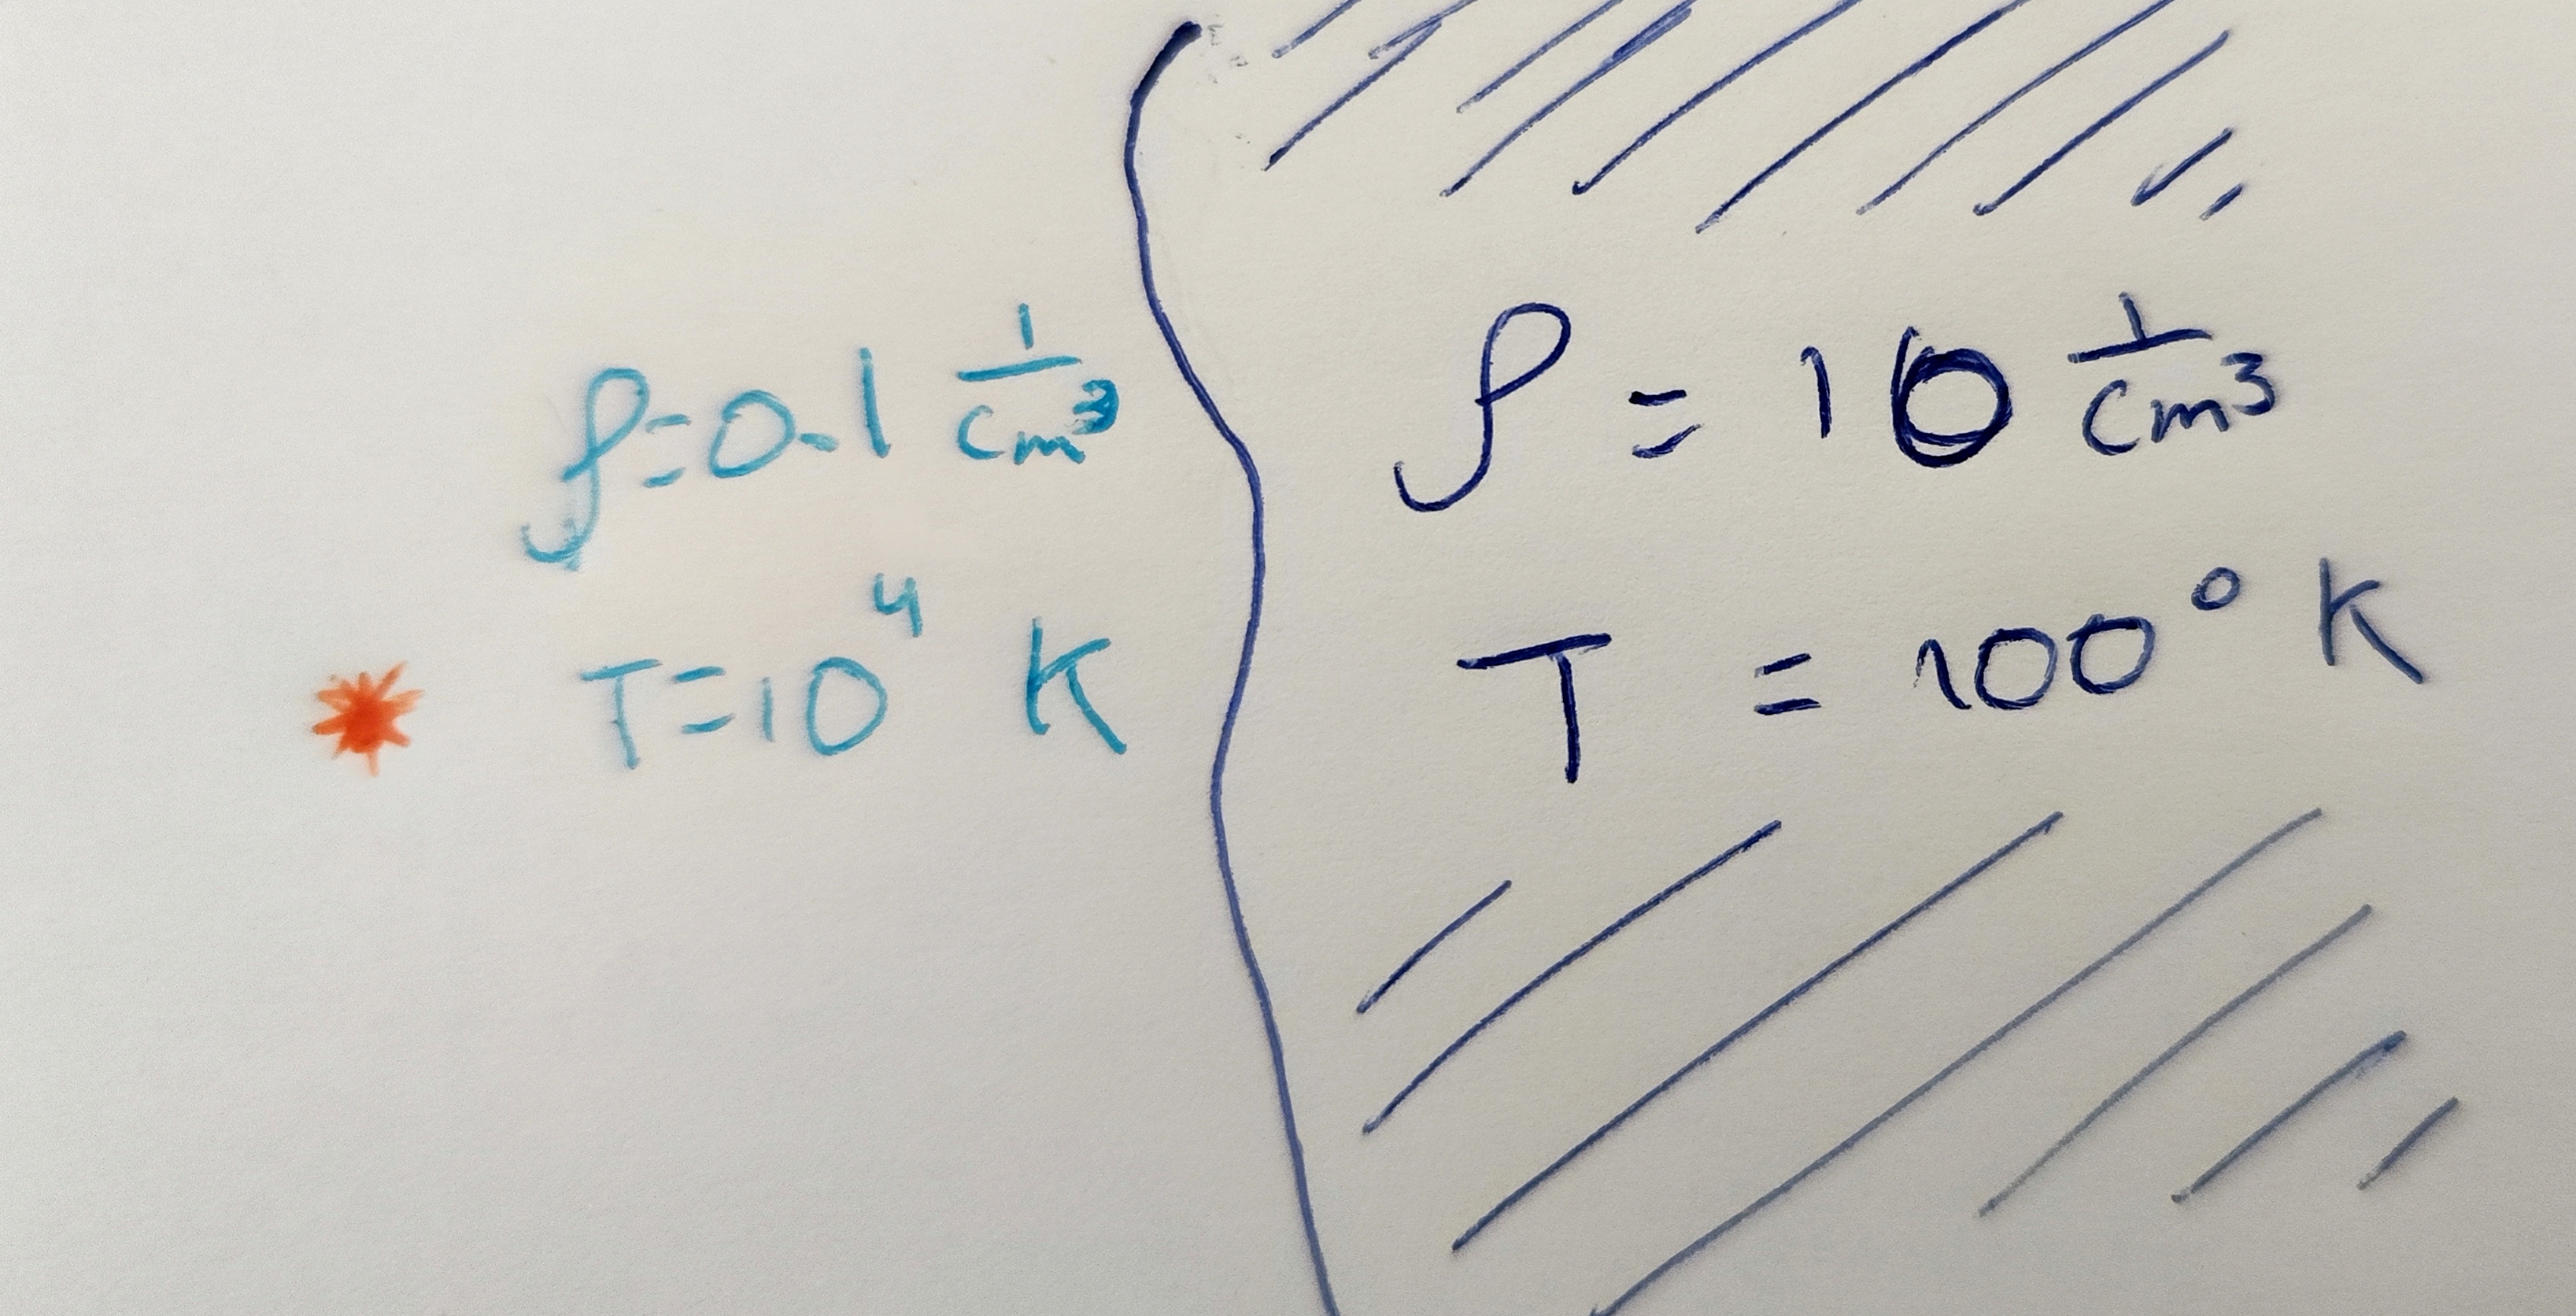
\includegraphics[width=0.5 \textwidth]{images Chapter 1/C1_Kahn.jpg}
    \caption{Esquema inicial utilizado en \cite{Kahn:1954}}
    \label{kahn_zones}
\end{figure}

Cuando la radiación UV comienza a calentar el gas de la nube, el gas ionizado comienza a expandirse en dirección a la estrella, esto ya que en esta dirección la densidad es menor que la de la nube y puede expandirse libremente. De esta manera mientras el gas ionizado va en dirección a la estrella, el frente de ionización se va alejando. A este efecto se le conoce como efecto rocket.

En un inicio esta radiación ioniza el gas a una tasa muy rápida causando una ``tormenta de partículas ionizantes'' que viene por parte de la nube, conforme esto va evolucionando se crea una capa aislante alrededor de la nube. Mientras esto ocurre hay un choque interno que va viajando a través de la nube a la parte trasera. Para que esto ocurra \cite{Kahn:1954} da cierto criterios, en los cuales dice que la radiación no debe ser muy débil o demasiado fuerte.

\section{Estrellas Wolf-Rayet y sus vientos}

Las estrellas Wolf-Rayet (WR) son estrellas evolucionadas de estrellas masivas, como estrellas tipo O, y fueron nombradas así después de que Charles Wolf y Georges Rayet identificaran 3 estrellas en Cygnus con sus  anchas líneas de emisión que las caracterizan muy bien. 

Estas estrellas se caracterizan por el cociente que hay entre sus líneas de emisión intensa que las caracterizan. \cite{Smith:1968} las clasifica principalmente como WN a aquellas que son abundantes en He y N, WC a las que son abundantes en He y C. Además les pone un número para identificar esencialmente si son tipo tardío o temprano.

\begin{table}[h!]
    \begin{center}
        \begin{tabular}{c c}
        \toprule
        \multicolumn{2}{c}{Clasificación de estrellas WR} \\ \midrule
        Clasificación    & Tipo de estrellas\\ \midrule
        WN2--5     & Tipo temprana, WNE (Early WN)\\
        WN7--9 & Tipo tardía, WNL (Late WN) \\
        WC4--6 & WCE\\
        WC7--9 & WCL \\ \bottomrule
        \end{tabular}
    \caption{Principal clasificación de estrellas WR  según sus líneas de emisión. Dentro de las WC, las que se clasifican como WC6 pueden ser de tipo tardía o temprana.}
    \label{tab:WR-clasificacion}
    \end{center}
\end{table}

También están las estrellas WO que son abundantes en He y O, pero en realidad son una extensión de las WCE. Para las estrellas en las que detectamos una cantidad considerable de H en su atmósfera se les pone también una ``h'' \citep{SSM:1996}.

Estas estrellas se caracterizan principalmente por sus fuertes vientos que pueden ser del orden de $\sim$\SI{1000}{km/s}, los cuales provocan sus líneas de emisión anchas. Así como también tienen una alta pérdida de masa $\sim$2--\SI{10e-5}{\msun/yr}. Típicamente son estrellas de 10--\SI{25}{\msun} que son descendientes de estrellas tipo O y se caracterizan por tener intensas líneas de emisión de libre-libre desde el $\mu$m hasta el cm \citep{crowther:2007}.

\section{Nebulosa M1-67}

M1-67 es la nebulosa alrededor de la estrella WR-124, que tiene índice espectral WN8h. En la figura \ref{fig:zones} vemos que la imagen tomada con el telescopio espacial Hubble (HST) en H$\alpha$ se puede notar una gran presencia de H en toda la nebulosa, mientras que en la imagen tomada por el telescopio espacia James Webb (JWST), tomada en varios filtros de los cuales incluye en  el infrarrojo cercano, podemos ver una gran estructura. Algo muy notorio a simple vista en la imagen de JWST es que podemos apreciar la presencia de algunos nudos en la nebulosa como se ve  en la figura \ref{fig:zones}.

\begin{table}[h]
    \centering
    \begin{tabular}{c c c}
        \toprule
        \multicolumn{3}{c}{Parámetros de la estrella WR 124} \\ \midrule
         D & \SI{5.429}{kpc} & J. Arthur, priv.~comm.\\
         $v_\infty$ & \SI{710}{km/s}  & \cite{Hamman:2006}\\
         $\dot{M}$ & \SI{2e-5}{M_\odot/yr} & ?\\
         L & \SI{1.25e49}{s^{-1}} & \cite{crowther:2007} \\
         $F_{H_\alpha}$ & \SI{3e-14}{erg.cm^{-2}.s^{-1}} & \cite{Grosdidier:1998}\\ \bottomrule
    \end{tabular}
    \caption{Parámetros de WR 124}
    \label{tab:parametros WR-124}
\end{table}

\begin{figure}[h]
    \centering
    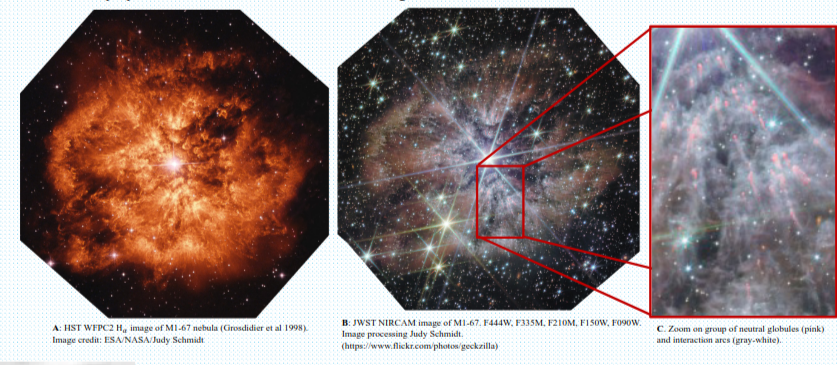
\includegraphics[width=0.75\textwidth]{images Chapter 1/C1_WR124.png}
    \caption{...}
    \label{fig:zones}
\end{figure}

Podemos ver como muchos detalles en cada uno de los filtros, en especial de como podemos ver en color rosa lo que parece ser choques de una gran acumulación de gas neutro que está interactuando con el viento de la estrella, y al rededor de ellos vemos una morfología similar a la de los proplyds que hay en otras nubes moleculares. También podemos ver como estos tienen una estela en la parte más lejana de la interacción, pero para nuestro estudio solo nos concentraremos solo en la parte más central.

\chapter{Modelos analíticos de flujos fotoevaporativos interactuando con una presión externa}
\chaptermark{Modelo analítico}

En este capitulo vamos a describir el modelo que se propone para explicar la interacción que hay entre el flujo fotoevaporativo por parte de los nudos que hay en la nebulosa M1-67 y el viento estelar por parte de la estrella WR-124. Para esto hemos considerado que ya han pasado todas las fases mencionadas en la sección \ref{Sec:fluijos fotoevaporativos} y ahora estamos en un equilibrio de ionización, por lo que el nudo no se comprimirá o expandirá en escalas significativas, es decir, que podemos considerar que el tamaño del nudo será constante. Podemos apreciar mejor la presencia de estos nudos en la figura \ref{fig:nudos}.

En esta interacción entre el flujo fotoevaporativo, el cual es supersónico, y el viento estelar se producen dos zonas chocadas y entre ellas una discontinuidad de contacto como se describe en la figura \ref{fig:zones}. De estas zonas esperamos ver solo el flujo fotoevaporativo chocado y no el viento estelar chocado ya que este último es menos denso además de que es no radiativo y la longitud de enfriamiento es más grande que la región de interacción

\begin{figure}[h]
    \centering    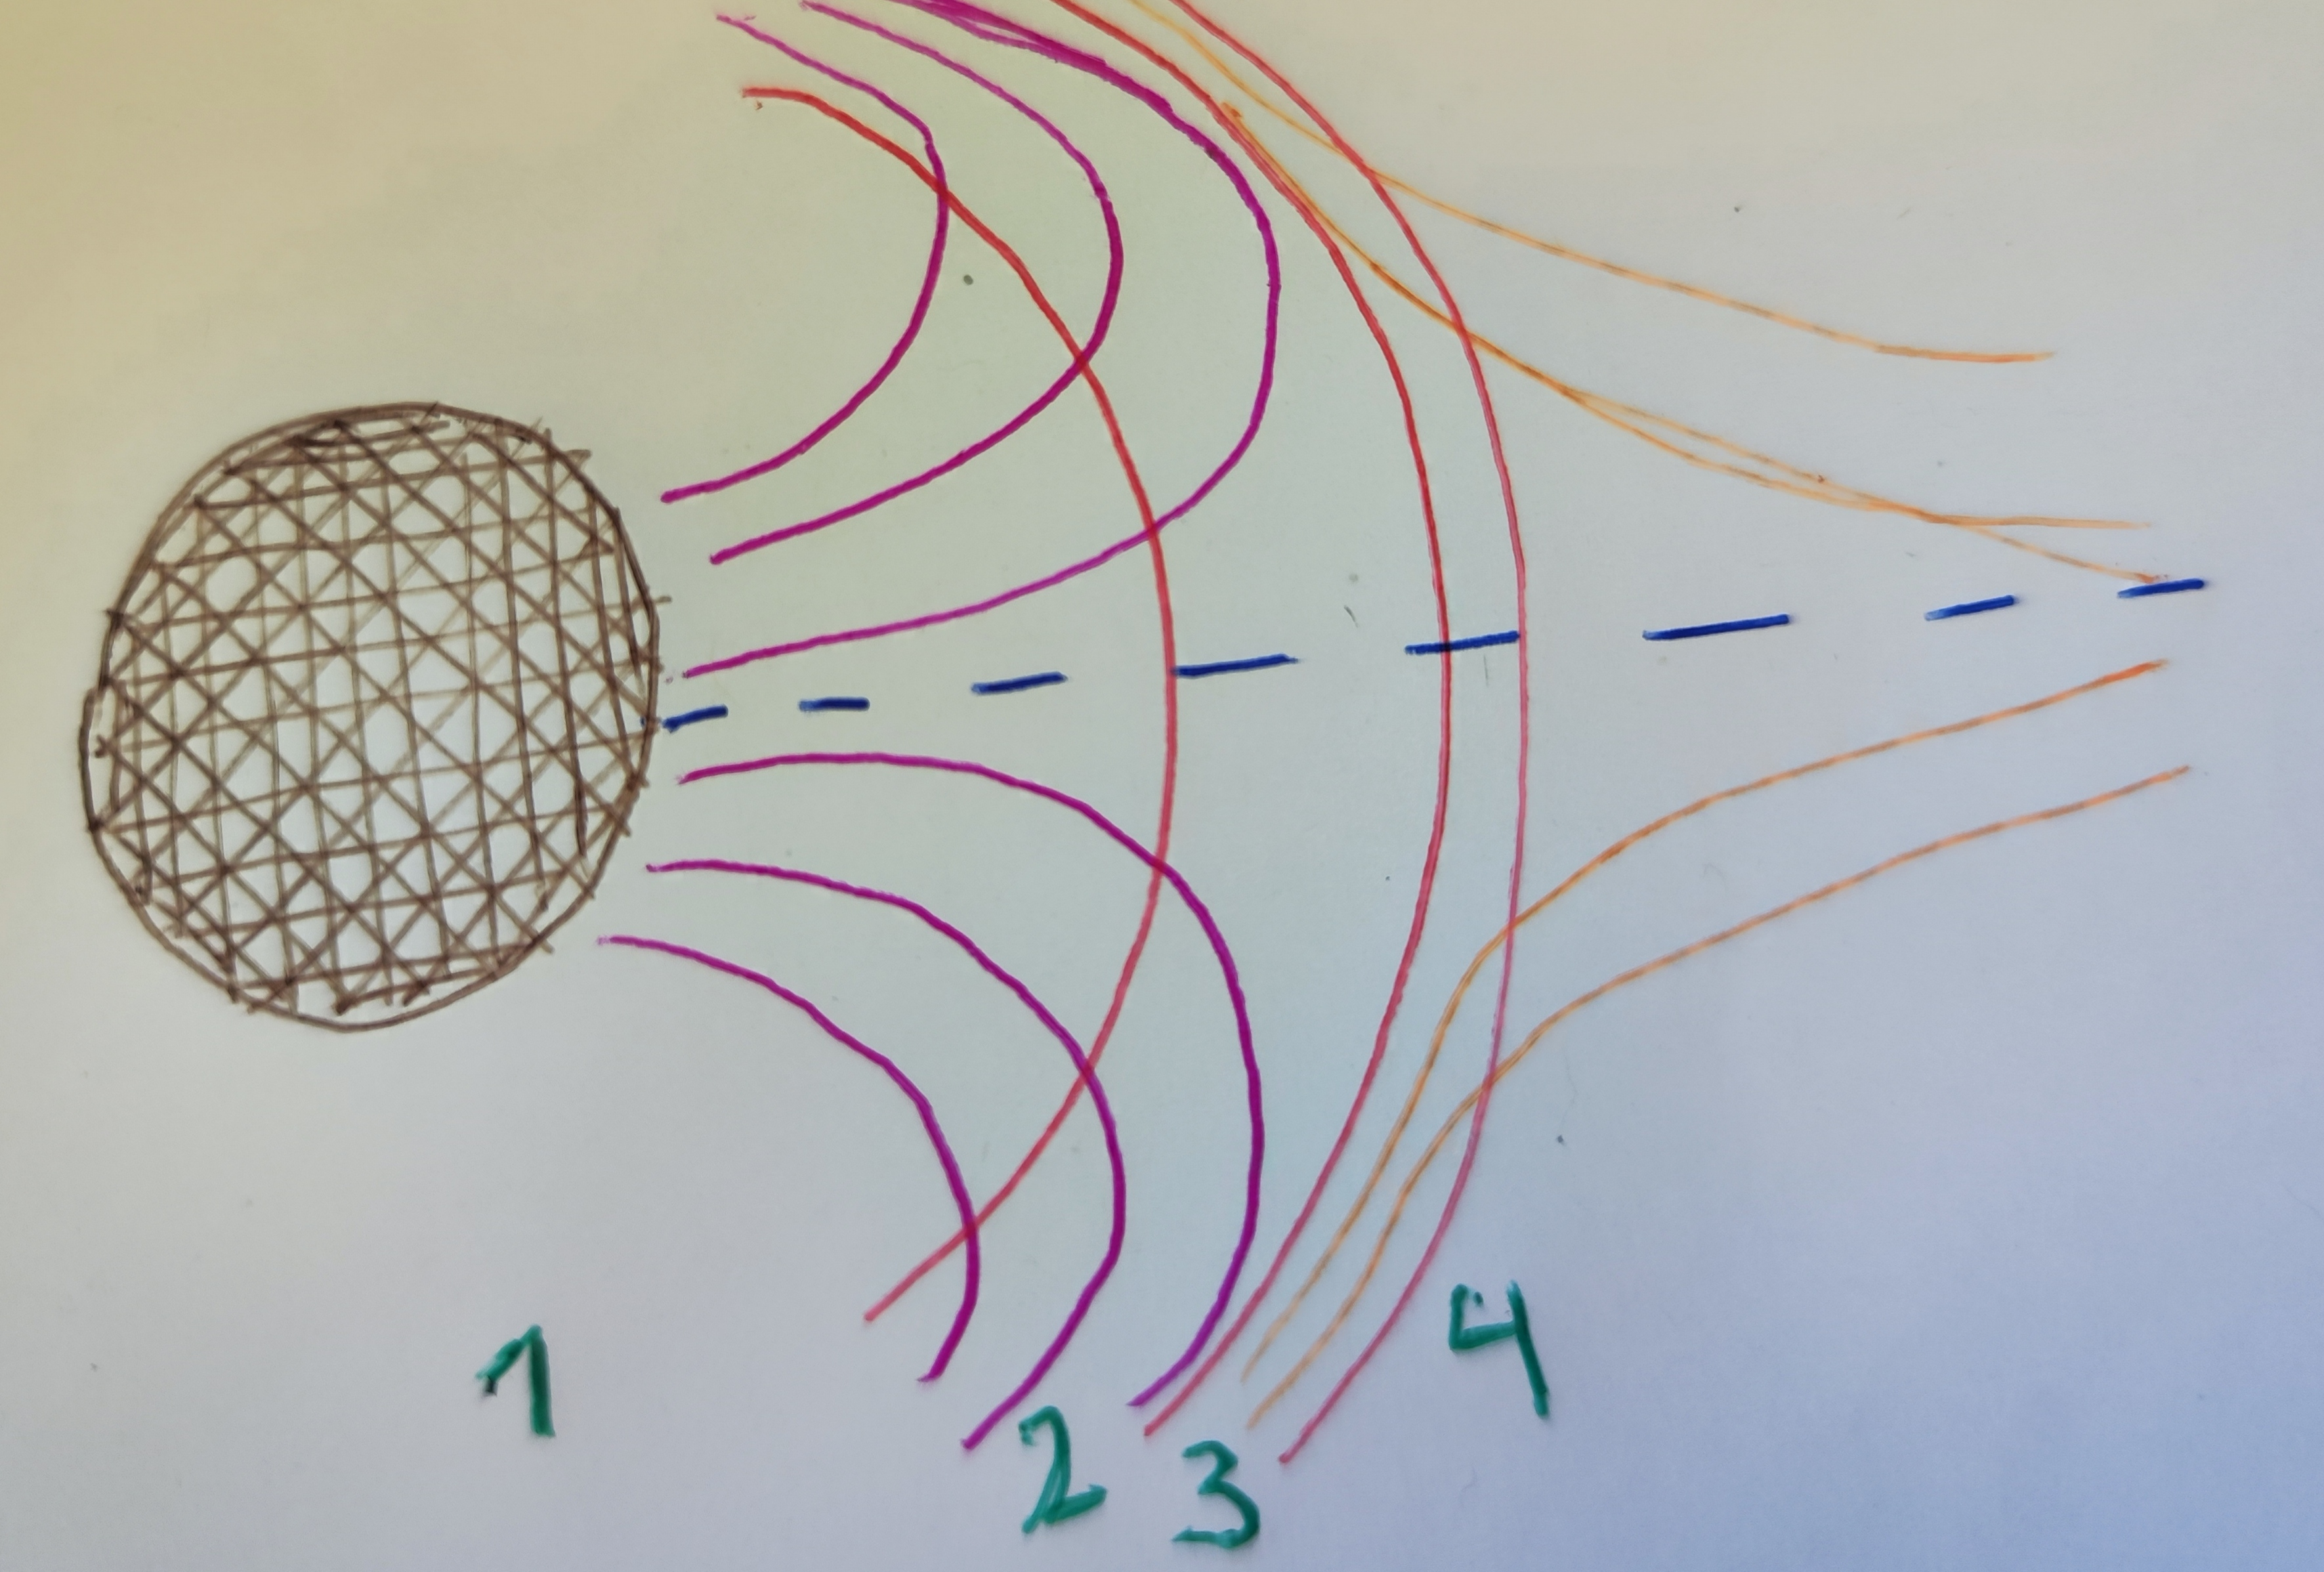
\includegraphics[width=0.75\textwidth]{images Chapter 2/Chp2_Zone.jpg}
    \caption{La interacción entre el flujo fotoevaporativo y el viento estelar de una estrella forma 4 zonas. La línea punteada une al glóbulo con la estrella y es el eje de simetría que vamos a considerar. La zona 1 es donde el flujo fotoevaporativo sale de la superficie del glóbulo con un número de Mach 1 y va aumentando, la zona 2 es el flujo fotoevaporativo chocado, la cual esperamos ver en las observaciones como una cáscara, la zona 3 es el viento chocado y la zona 4 es donde viaja el viento estelar supersónico, el cual es menos denso que el flujo fotoevaporativo.}
    \label{fig:zones}
\end{figure}

En este modelo tenemos la ventaja que podemos considerar un eje de simetría como vemos en la figura \ref{fig:zones} y alrededor de este podemos considerar una simetría cilíndrica como se ve en la figura \ref{fig:cilinders}, de esta manera podemos ignorar los movimientos transversales y tratarlo más como un problema radial.


\begin{figure}[h]
    \centering    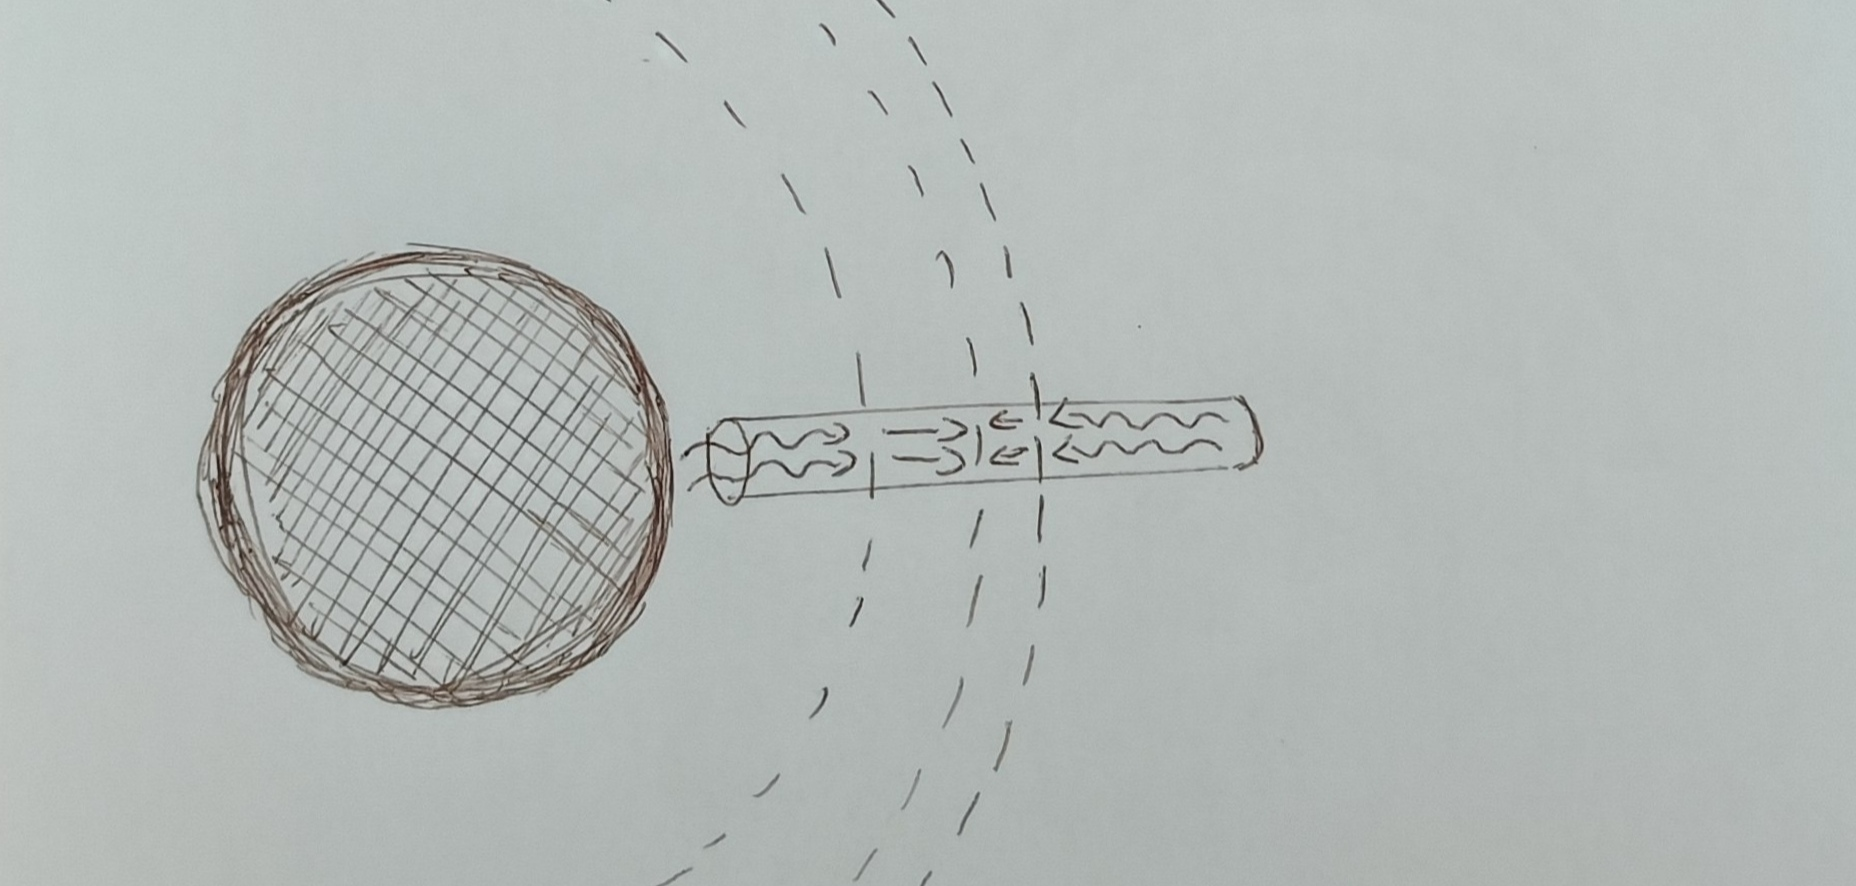
\includegraphics[width=0.75\textwidth]{images Chapter 2/Chp2_cilinders.jpg}
    \caption{Si consideramos una simetría cilíndrica con un radio muy pequeño, podemos tratar este problema de manera radial y de tal manera que la radiación y el viento estelar inciden de manera perpendicular al glóbulo.}
    \label{fig:cilinders}
\end{figure}

\section{Estimación de la densidad ionizada a partir del brillo superficial de $H_\alpha$}

Para estimar la densidad ionizada, usamos primero la definición de medida de emisión (EM por sus siglas en inglés)
\[EM=\int_z n_i n_edz\] donde en este caso estaremos integrando sobre nuestra línea de visión. Esta EM depende tanto de la densidad de electrones como de iones, pero en nuestro caso vamos a considerar un equilibrio de ionización entre el flujo fotoevaporativo y el viento estelar, por lo que $n_e=n_i$.

\begin{figure}
    \centering    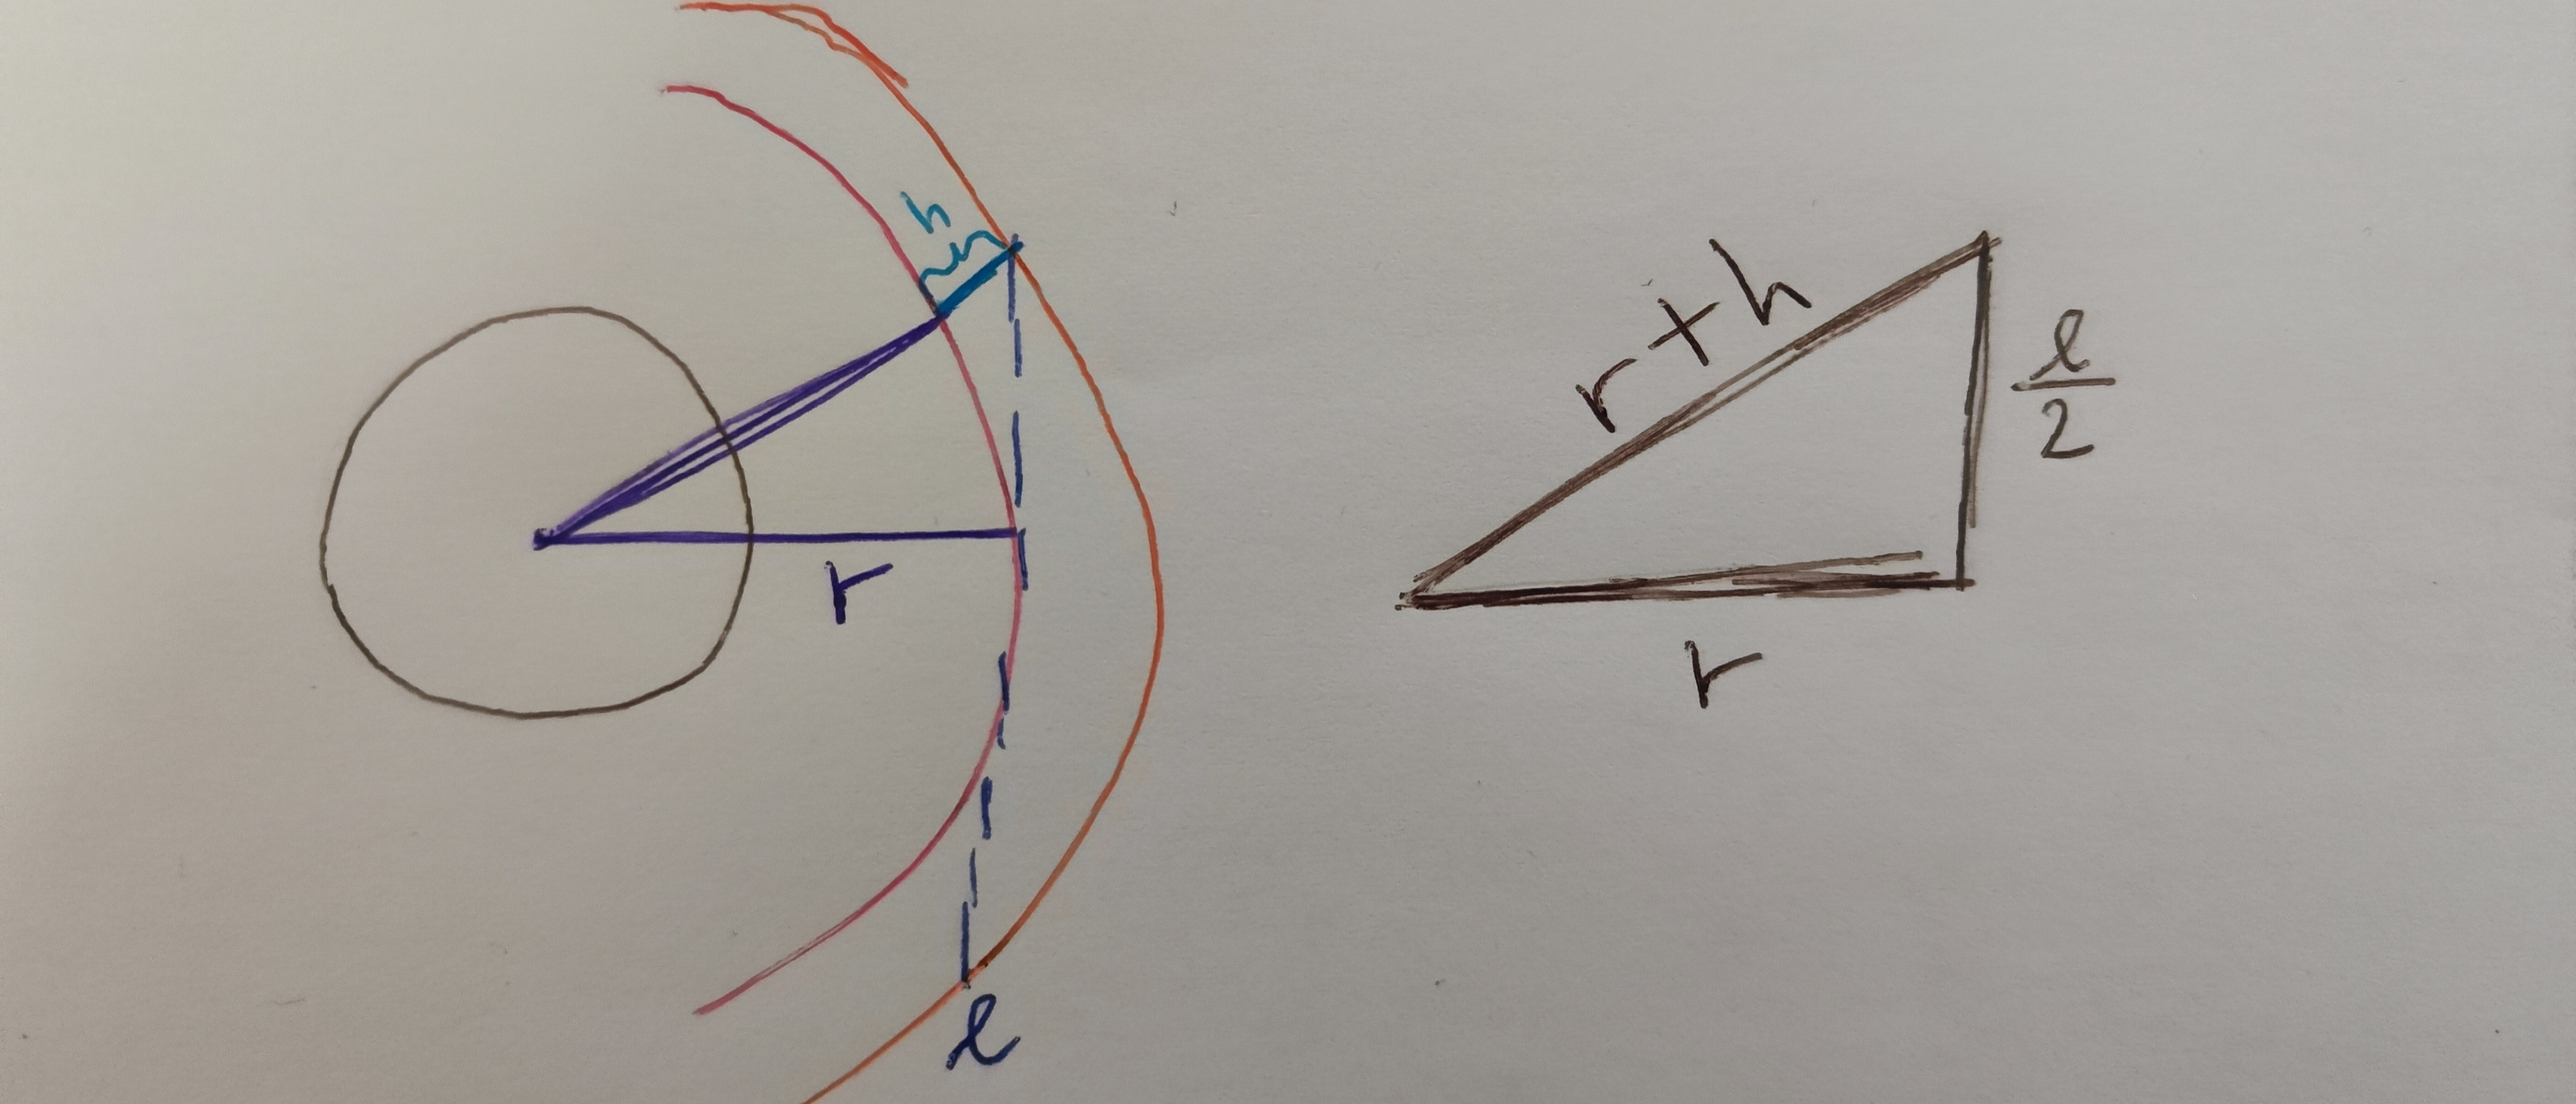
\includegraphics[width=0.75\textwidth]{images Chapter 2/C2_EM.jpg}
    \caption{Como la medida de emisión se mide a lo largo de la línea de visión, vamos a tener un máximo en la línea punteada $l$ y si consideramos una simetría esférica vamos a tener esta configuración donde $h$ será el ancho de la cáscara chocada, $r$ el radio del centro del glóbulo hasta donde inicia el flujo fotoevaporativo chocado y $h<r$.}
    \label{fig:EM}
\end{figure}

Si suponemos una simetría esférica entre esta interacción del flujo fotoevaporativo y el viento estelar, podemos tomar, por geometría, que
\[EM=2\sqrt{2rh}n^2.\]


Esto ya que de la figura \ref{fig:EM} tenemos que por geometría $r^2+\Big(\frac{l}{2}\Big)^2=(r+h)^2=r^2+2rh+h^2\approx r^2+2rh\Rightarrow l=2\sqrt{2rh}$. De esta manera, usando la EM tenemos que \[n=\sqrt{\frac{EM}{l}}=\sqrt{\frac{EM}{2\sqrt{2rh}}}\] 

\section{Modelo hidrodinámico estacionario}

Para este modelo es importante mencionar que no estamos considerando ninguna fuerza de gravedad por parte de la estrella o del mismo glóbulo, ver apéndice \ref{App:fuerzas}, así como tampoco vamos a considerar campos magnéticos por simplicidad.

Vamos a considerar equilibrio de ionización ya que ya que como vimos en la sección \ref{Sec:fluijos fotoevaporativos} el tiempo en que se forma la capa aislante formada por la radiación UV es muy corto mientas que el tiempo en que tenemos esta interacción entre el flujo fotoevaporativo y el viento estelar es lo suficientemente grande como para considerar este modelo como estacionario.

Como ya se mencionó antes, podemos tener una simetría cilíndrica alrededor del eje de simetría que une al glóbulo con la estrella. De esta manera podemos ignorar los movimientos transversales ya que los gradientes en estas direcciones son muy pequeñas si los comparamos con los gradientes en la dirección axial.

\begin{figure}[h]
    \centering    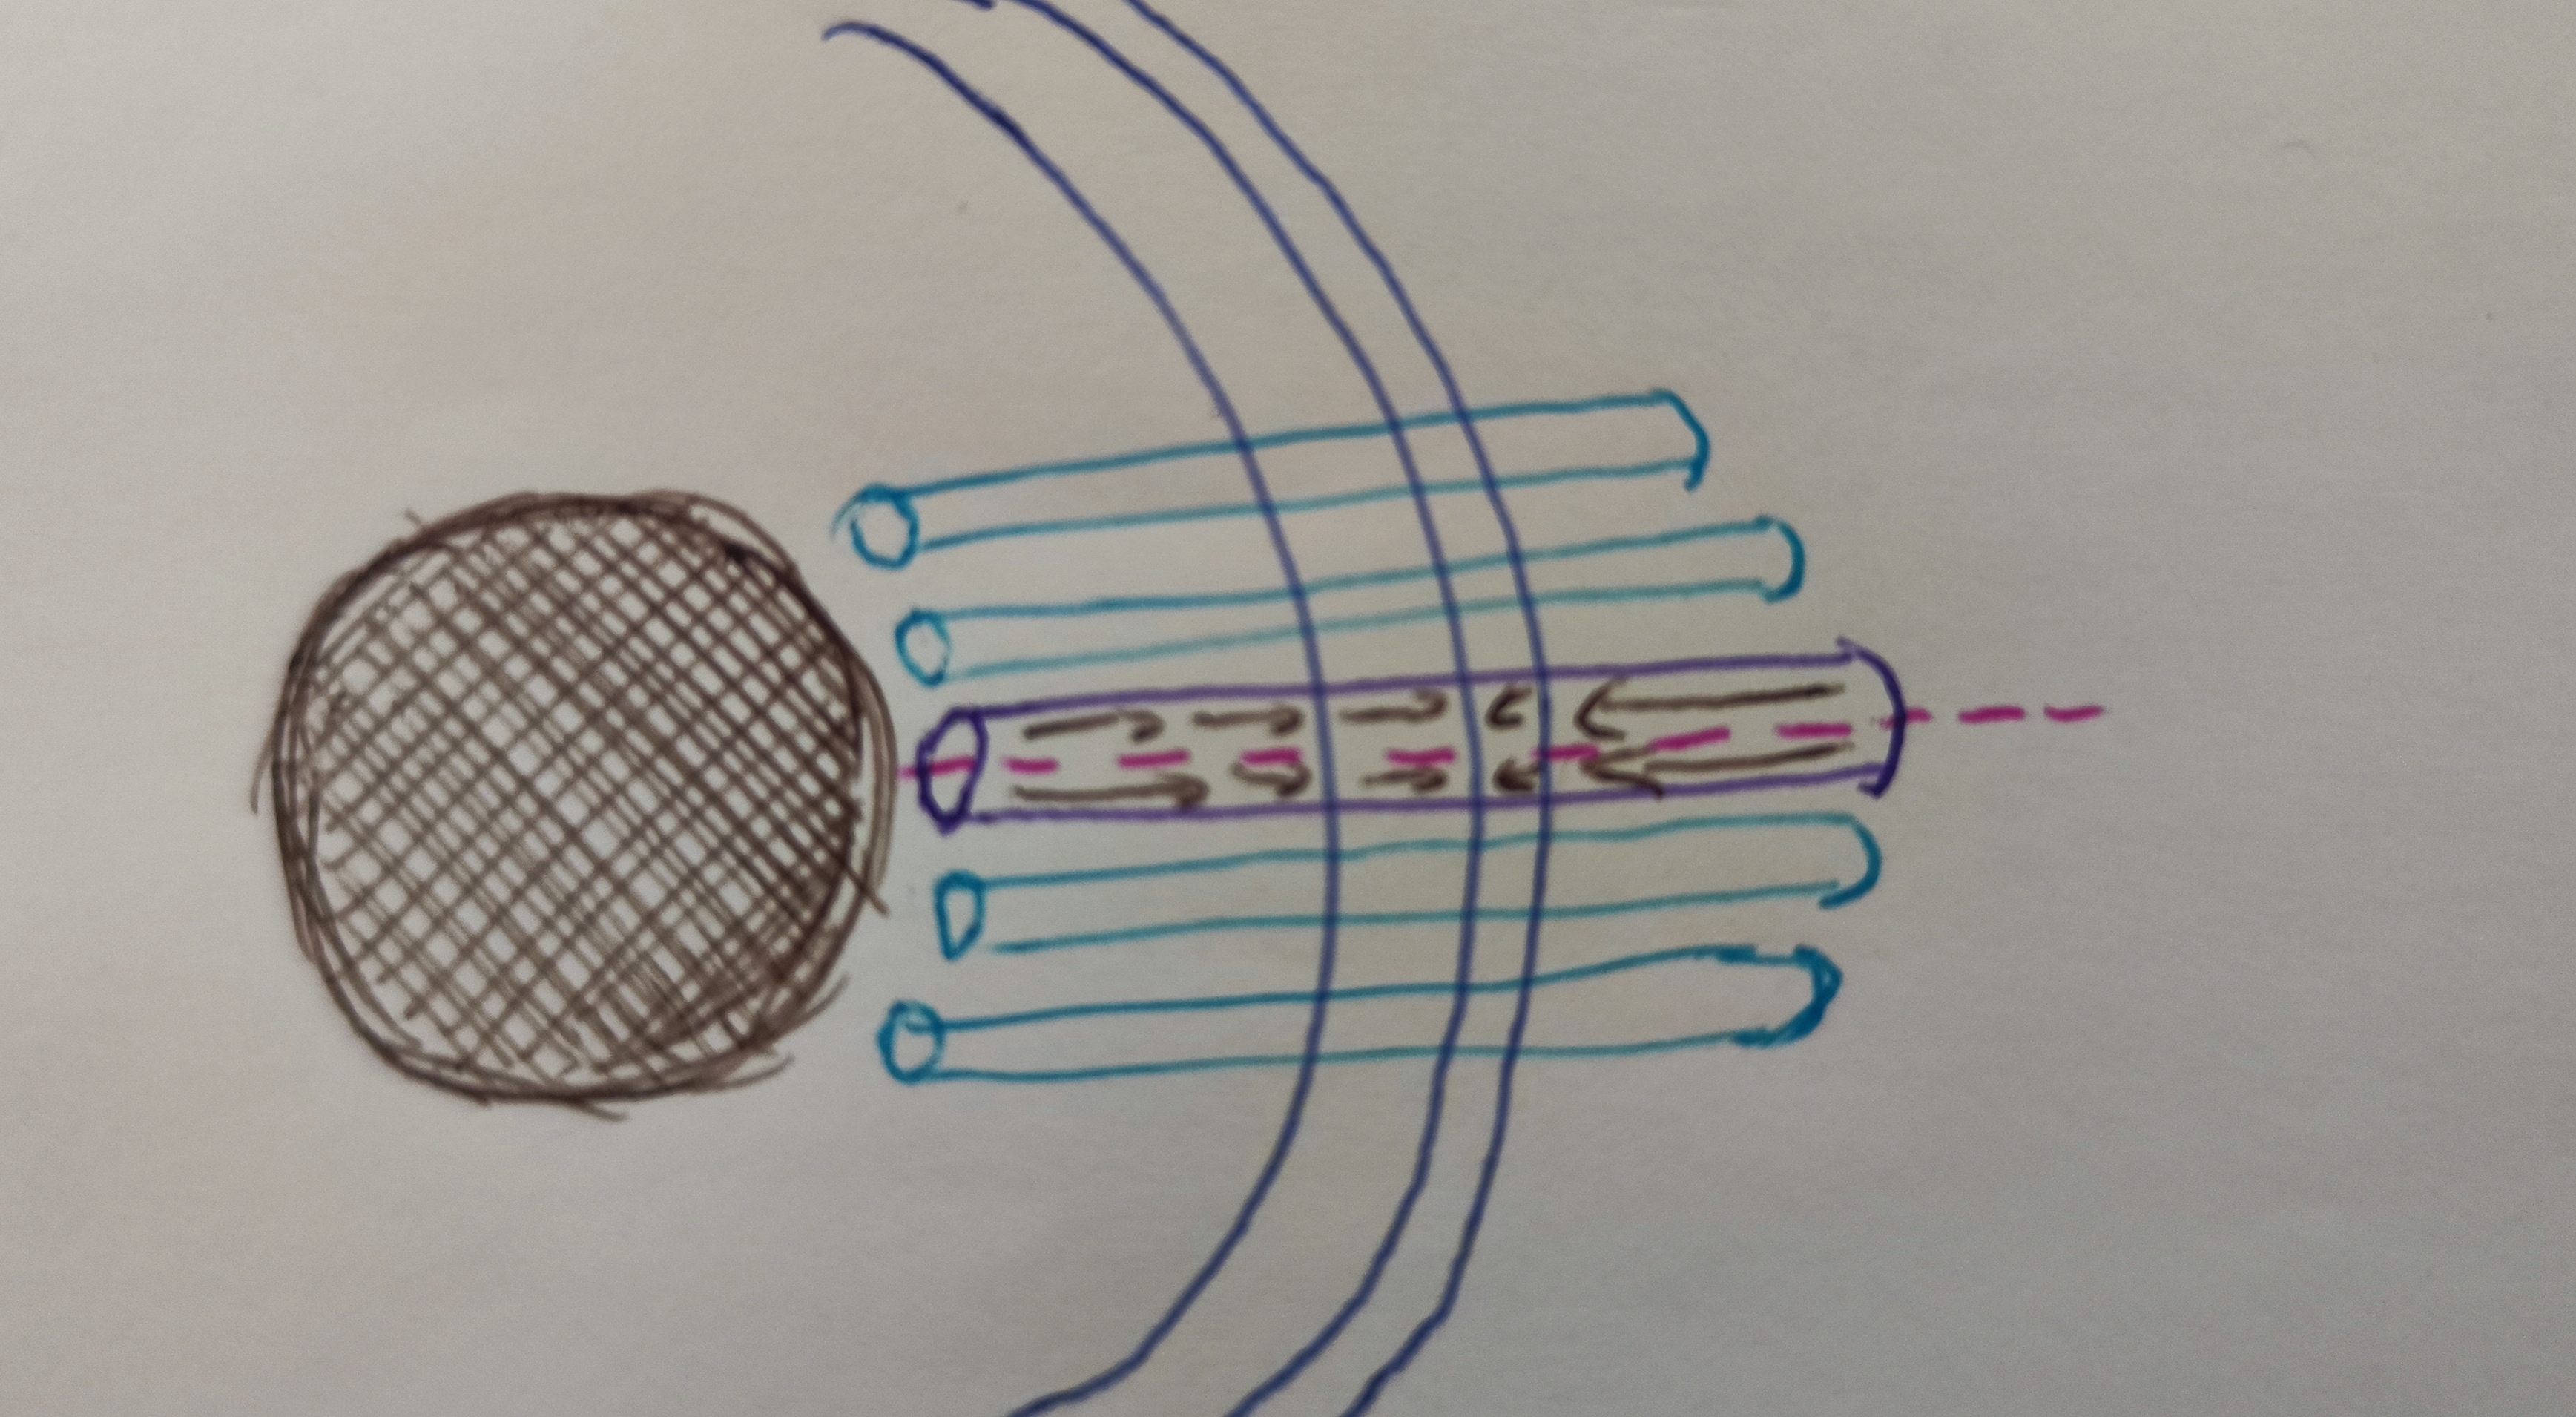
\includegraphics[width=0.75\textwidth]{images Chapter 2/C2_cilindersfamily.jpg}
    \caption{Descripción de la familia de cilindros que vamos a tener a cada ángulo y de los cuales solo va considerar el cilindro de color azul intenso el cual está en el eje de simetría para tomar el problema de manera radial.}
    \label{fig:cilindross}
\end{figure}

En realidad vamos a tener una familia de cilindros a cada ángulo como vemos en la figura \ref{fig:cilindross}, pero con lo anterior mencionado vamos a tener que el flujo que pasa a través de un cilindro es independiente de los demás, por lo que nos podemos enfocar solo en aquel que está en el eje de simetría donde tanto la radiación como el viento estelar vana a incidir de manera radial en la superficie del glóbulo y entonces podemos pasarlo solo a un problema radial.

Para el flujo fotoevaporativo por parte del glóbulo vamos a considerar las ecuaciones de hidrodinámica, la ecuación de conservación de masa ya que como dijimos antes, el tiempo en el que un bulto sale de esta interacción le toma bastante tiempo. Usaremos también la ecuación de Bernoulli para un gas isotermo, donde la velocidad del sonido en este gas dependerá de la temperatura.

% Balance between ionizations and recombinations

\section{Ecuación de estado y equilibrio de ionización}

En este modelo tenemos ciertas condiciones iniciales para el flujo fotoevaorativo, como ya dijimos este flujo es supersónico por lo que inicialmente sale de la superficie del glóbulo con un número de Mach igual a 1 y este va aumentando conforme atraviesa toda la zona 1 de la figura \ref{fig:zones}. En principio podríamos tomar que tanto el radio del glóbulo como la densidad en su superficie son parámetros libres, pero con las observaciones podemos medir el radio y la densidad la podemos calcular ya que esta debe ser consistente por haber considerado equilibrio de ionización.

Con este modelo se pretende ver hasta donde llegamos a un equilibrio de presión entre la presión por parte del flujo fotoevaporativo y a presión RAM del viento estelar. Para el caso de la presión del flujo fotoevaorativo vamos a considerar tanto la presión térmica como la hidrodinámica por lo que la presión total está dada por
\[P_{tot}=P_{ter}+P_{hid}=n\bar{m}c_s^2+n\bar{m}u^2=\rho c_s^2(1+M^2)\]
En este caso no estamos considerando presión magnética ni de radiación.

\begin{figure}[h]
    \centering 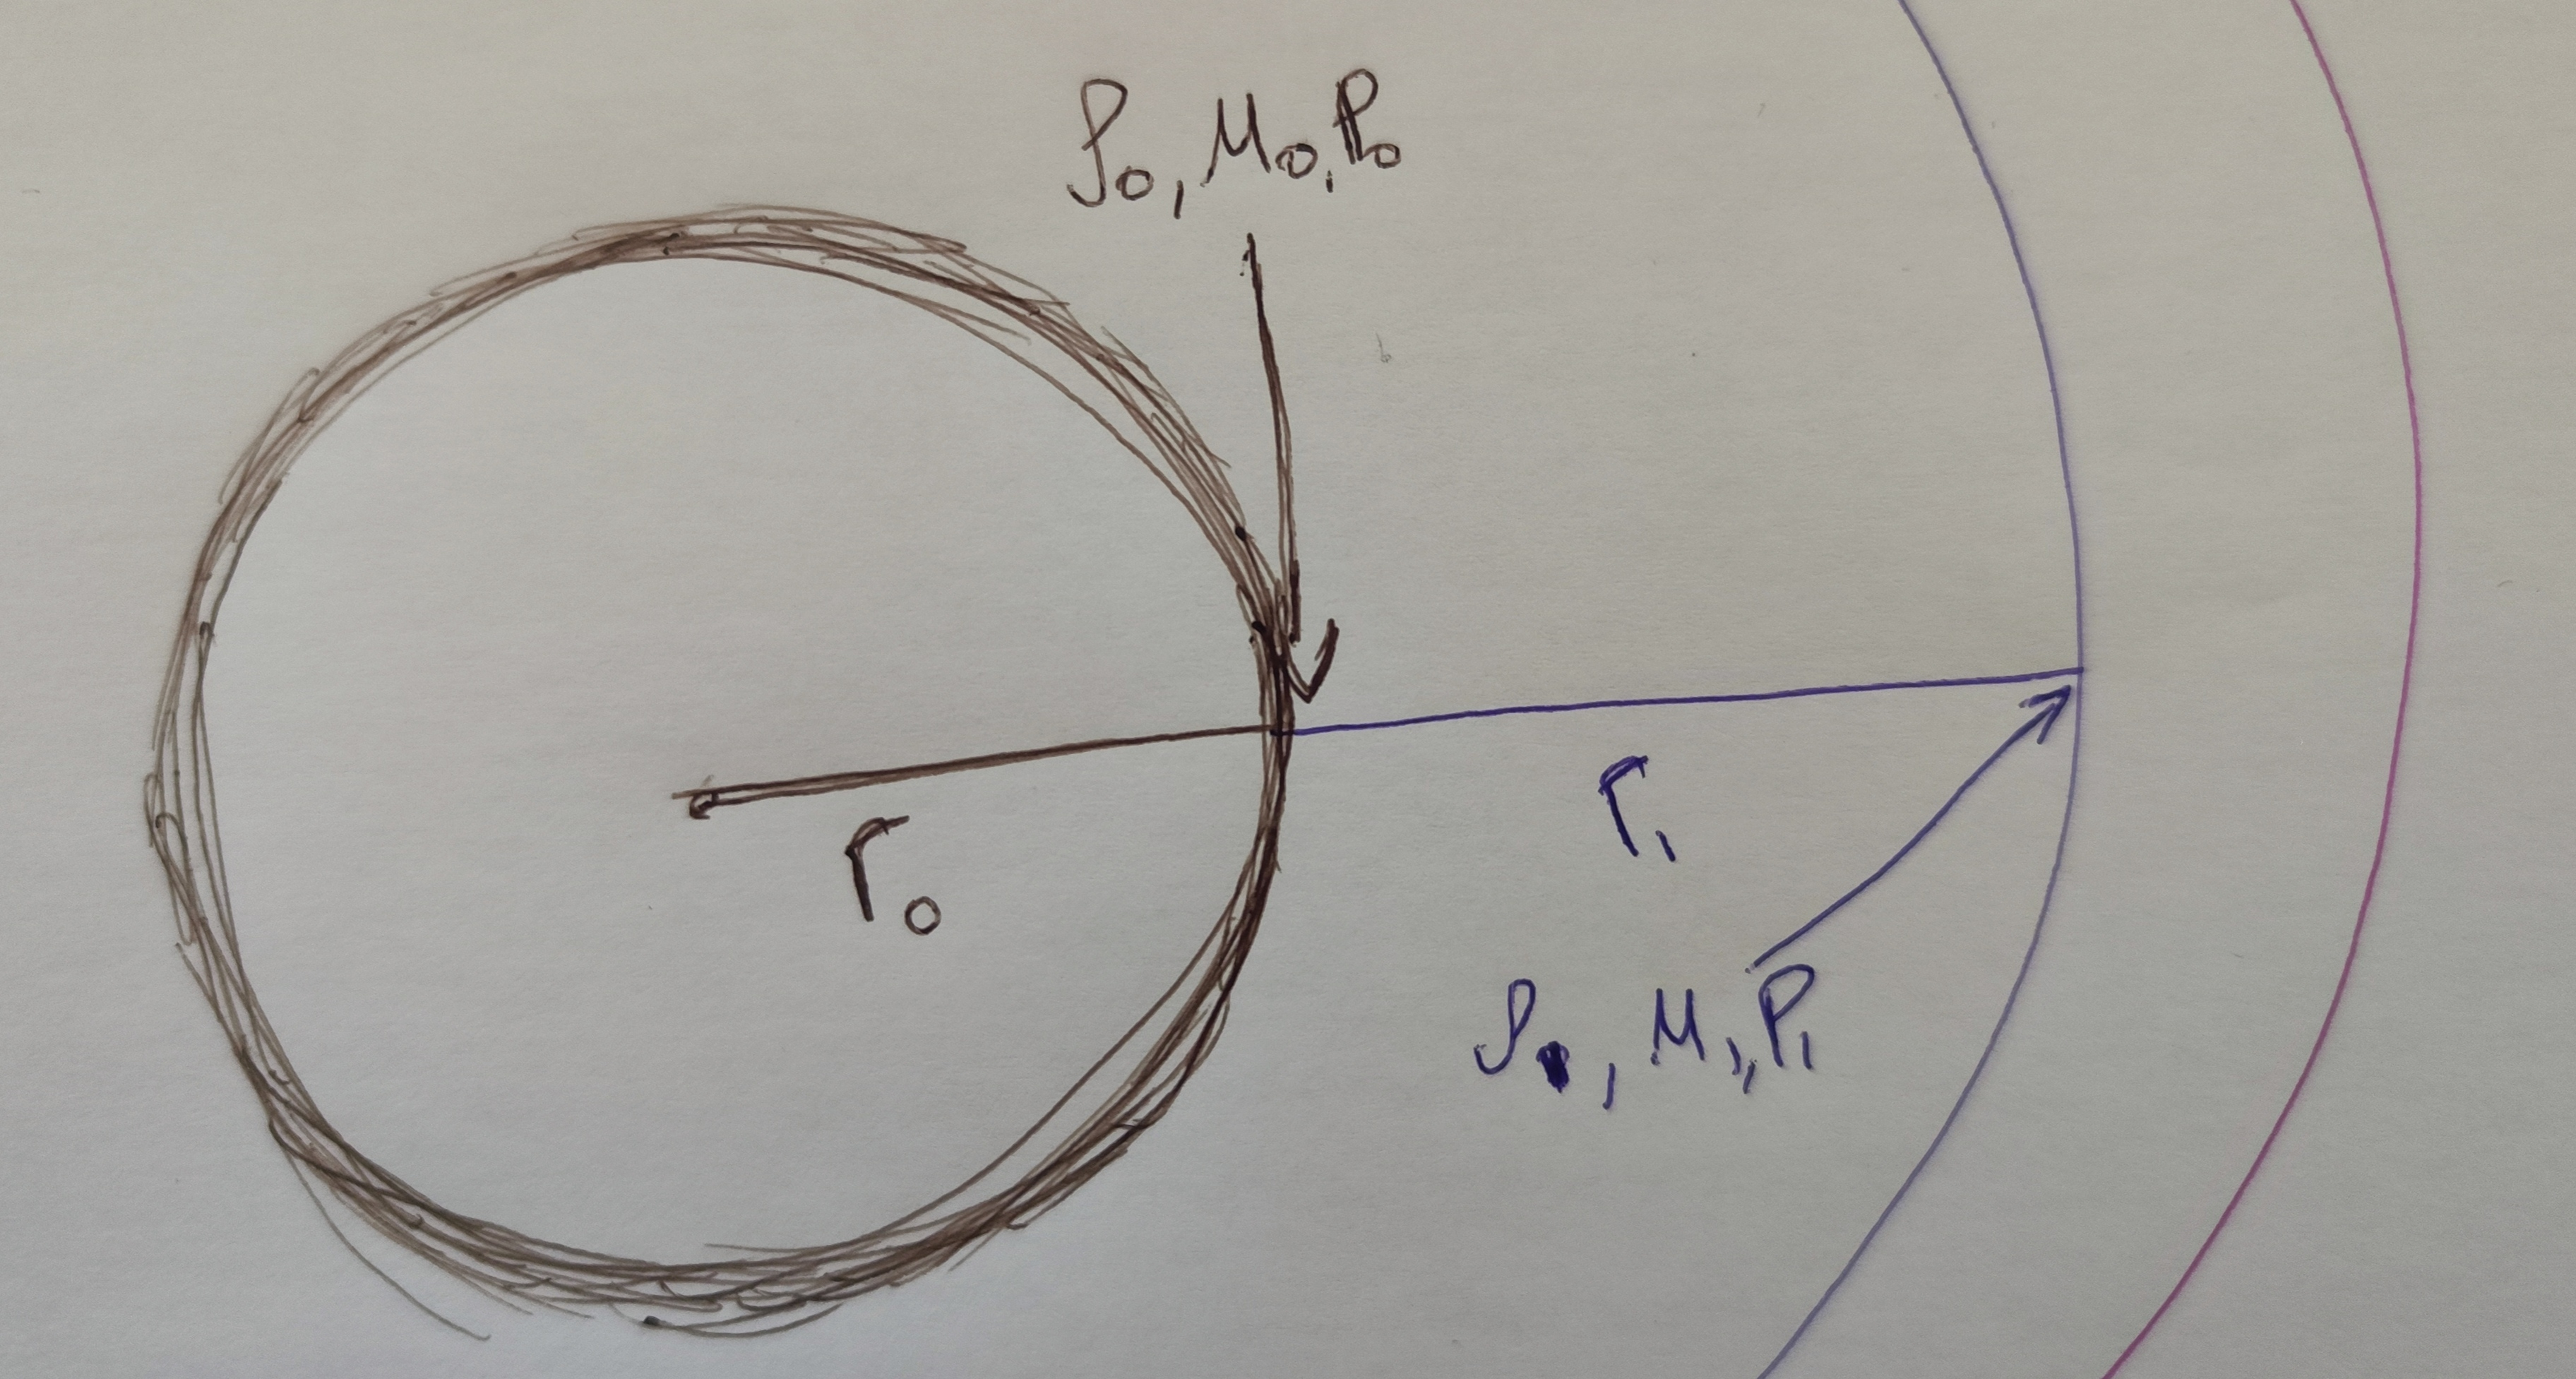
\includegraphics[width=0.75\textwidth]{images Chapter 2/C2_parameters.jpg}
    \caption{$r_0$ es el radio del glóbulo, mientras que $\rho_0,M_0$ y $P_0$ son los valores que tenemos en la superficie del glóbulo y conforme estos avanzan con dirección a la estrella sus valores van cambiando hasta tener valores $r_1$, que el radio del centro del glóbulo hasta la base del flujo fotoevaporativo chocado, $\rho_1,M_1$ y $P_1$ que son los valores que tendrán en la base del flujo fotoevaporativo chocado.}
    \label{fig:parameters}
\end{figure}

Este equilibrio de presión se logrará a un radio $r_1$ que es donde la presión del flujo fotoevaporativo ha disminuido un fracción $f$ de lo que era la presión inicial. Por lo que la presión cambia como 
\[f=\frac{P}{P_0}=\frac{\rho c_s^2(1+M^2)}{\rho_0 c_s^2(1+1)}=\frac{\rho}{\rho_0}\frac{1+M^2}{2}\]
Considerando la ecuación para la conservación de masa tenemos que
\[\rho r^2M	=\rho_0 r_0^2\]
y finalmente si consideramos la ecuación de Bernoulli isotérmica 
\[\frac{v^2}{2}+c_s^2\ln\rho=constante\]
tenemos que 
\[\frac{r}{r_0}=M^{-1/2}e^{\frac{M^2-1}{4}}\]
Ahora que tenemos tres ecuaciones y tres incógnitas podemos resolver, en nuestro caso lo hicimos de manera numérica. Al resolver estas ecuaciones para diferentes $f$ tenemos que tanto la presión como la densidad decaen con el radio, mientras que el número de Mach aumenta como vemos en la figura \ref{fig:grafica_C2}.

\begin{figure}[h]
    \centering    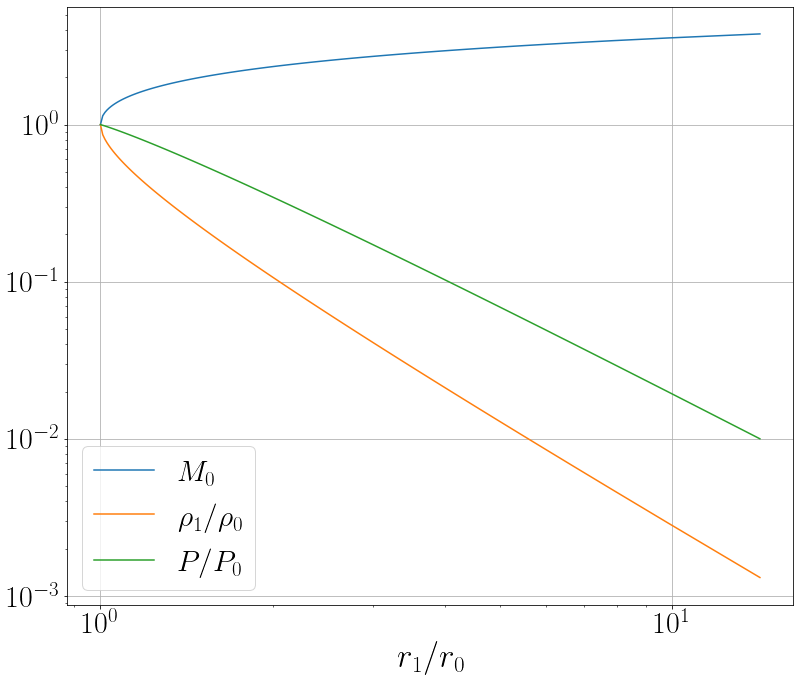
\includegraphics[width=0.75\textwidth]{images Chapter 2/C2_results.png}
    \caption{Gráfica de M, $\rho$ y $P$ normalizados como función de radio normalizado}
    \label{fig:grafica_C2}
\end{figure}

% Assumption of isothermal equation of state

% General solution for the internal structure of model


\chapter{Aplicación a M1-67}

Ahora vamos a aplicar este modelo a los nudos que hay en la nebulosa M1-67 y que interactúan con el viento estelar de la estrella WR-124.

De las observaciones vemos que estos nudos tienen tamaños típicos de 200--300 mili arco segundos de diámetro que son relativamente pequeños si los comparamos con la nebulosa planetaria que es de unas decenas de arco segundos. Estos nudos se encuentran típicamente a unos 10--30 arco segundos de la estrella.

\section{Observaciones con HST}

Para las observaciones del HST usamos los datos del proyecto HLA, utilizando el instrumento WFPC2 que observó en el filtro F656N, el cual se encuentra en el óptico, con un tiempo de exposición de \SI{4200}{sec}. Estos archivos son tipo imagen en formato FITS con un nivel de calibración 3.

\begin{figure}
    \centering
    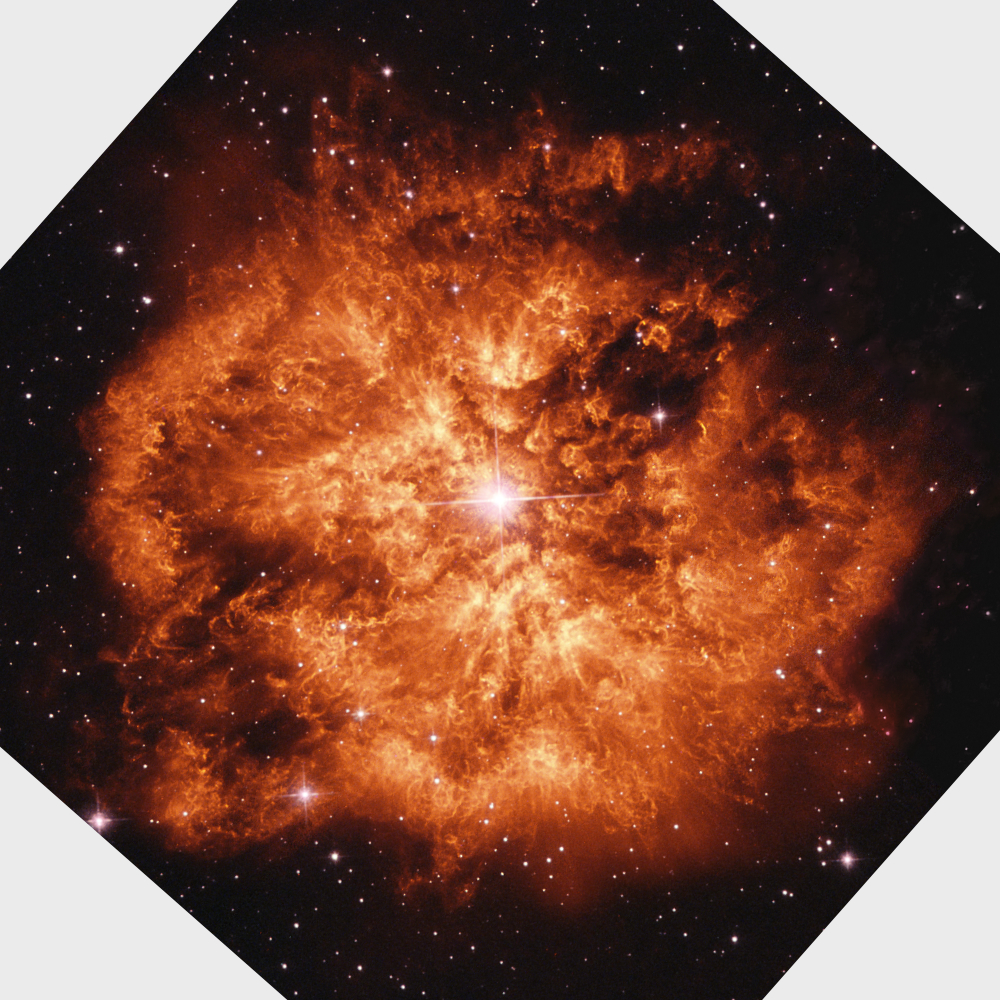
\includegraphics[width=0.75\textwidth]{m1-67-comp-full-hst.jpg}
    \caption{Imagen de M1-67 con el filtro H$\alpha$ \citep{Grosdidier:1998}.}
    \label{fig:M1-67HST}
\end{figure}

\section{Observaciones con JWST}

tiene unidades de brillo superficial MJr/sr.


\begin{figure}
    \centering
    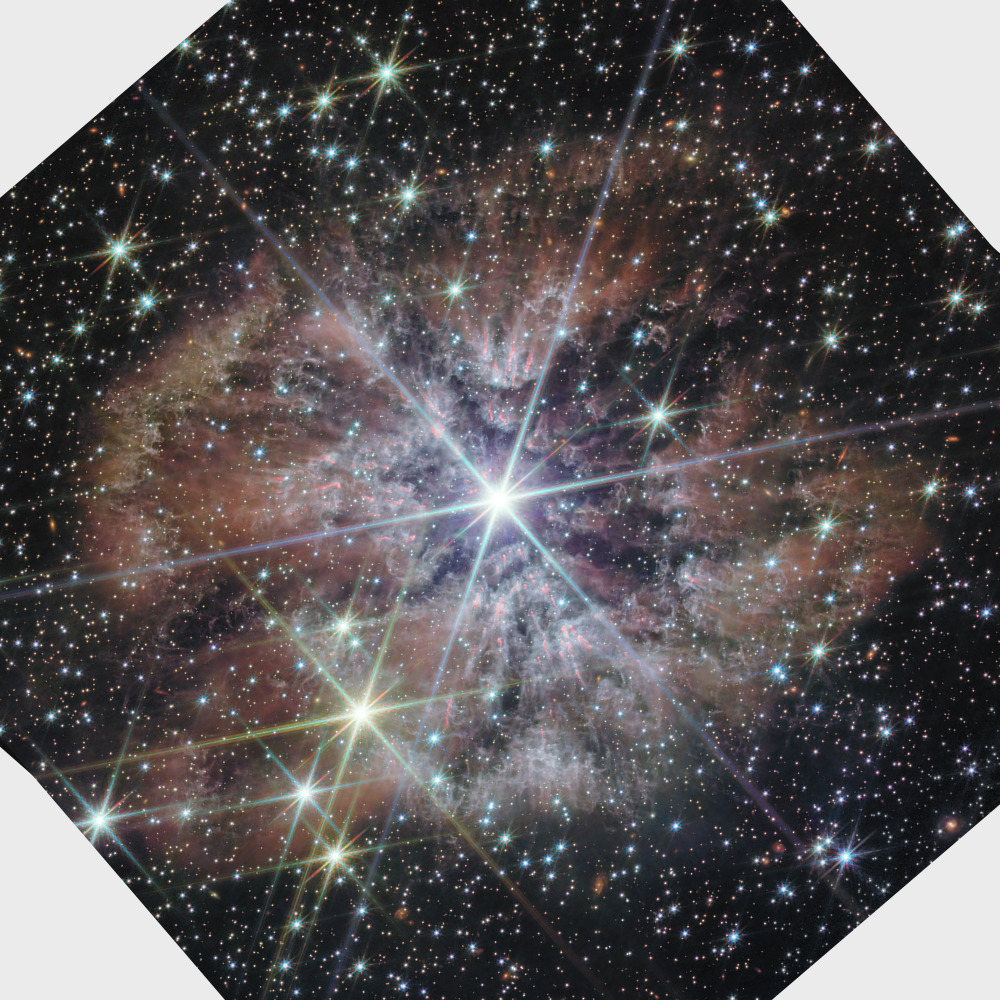
\includegraphics[width=0.75\textwidth]{M1-67-JWST.jpg}
    \caption{Imagen de M1-67 con JWST}
    \label{fig:M1-67JWST}
\end{figure}

\section{Ajustando el modelo a los perfiles de brillo radial}

Gracias a la gran resolución del JWST podemos saber donde se encuentran esto nudos exactamente. Con esto podemos identificar el eje de simetría que une al nudo con la estrella y con ello identificar mejor cual es la parte neutra del nudo y cual es la cascara chocada.

Para saber estos tamaños graficamos la intensidad de cada píxel como función de la distancia al centro del nudo. Para esto consideramos solo los píxeles que están a una distancia máxima de \SI{1.5}{arcsec} y a un ángulo máximo de 60 grados con respecto al eje de simetría.

A estos puntos les ajustamos dos gaussianas y una constante. La primer gaussiana será centrada en cero, que es el centro del nudo. Está primer gaussiana nos dirá el tamaño de la parte neutra del nudo. La segunda gaussiana se ajusta a la cáscara chocada donde tenemos otro pico de emisión debido a las recombinaciones que hay en esa región.

Para este ajuste le dimos menos peso a los píxeles que están mas lejanos del centro del glóbulo y que tienen un gran ángulo con respecto al eje de simetría.

\section{Estimando la presión RAM del viento estelar}

\section{Estimando la tasa de foto ionización}

\chapter{Conclusiones}

\appendix
\chapter{Estimación de fuerzas en el modelo} \label{App:fuerzas}

\bibliography{references}

\end{document}
